%%%% Small single column format
\documentclass[anonymous=false, %
               format=acmsmall, %
               review=true, %
               screen=true, %
               nonacm=true]{acmart}

\usepackage[ruled]{algorithm2e}
%\usepackage{parskip}
\usepackage{subcaption}
\usepackage{fontawesome}
\usepackage{footnote}
\makesavenoteenv{tabular}
\makesavenoteenv{table}
\usepackage{tabularx}

\urlstyle{tt}
\citestyle{acmauthoryear}

\begin{document}

\title{{ArviZ}: backend agnostic exploratory analysis of
{Bayesian} models in {Python}}

\author{Oriol Abril}
\orcid{0000-0002-1847-9481} % chktex 8
\affiliation{%
  % \institution{Universitat Pompeu Fabra}
  % \department{Department of Brain and Cognitive Sciences}
  %\streetaddress{43 Vassar St}
  % \city{Barcelona}
  %\state{MA}
  %\postcode{02139}
  %\country{USA}
}
\email{oriol.abril.pla@gmail.com}

\author{Colin Carroll}
\orcid{0000-0001-6977-0861}  % chktex 8
\affiliation{%
  \institution{PyMC3}
  %\streetaddress{625 Mt Auburn St #3}
  %\city{Cambridge}
  %\state{MA}
  %\postcode{02138}
  %\country{USA}
}
\email{colcarroll@gmail.com}

\author{Ari Hartikainen}
\orcid{0000-0002-4569-569X}  % chktex 8
\affiliation{%
  \institution{Aalto University}
  \department{Department of Civil Engineering}
  \city{Espoo}
  \country{Finland}
}
\email{ari.hartikainen@aalto.fi}

\author{Ravin Kumar}
\orcid{0000-0003-0501-6098}  % chktex 8
\affiliation{%
%   \institution{Northeastern University}
%   \department{Khoury College of Computer Sciences}
  %\streetaddress{360 Huntington Ave}
  % \city{Boston}
  % \state{MA}
  %\postcode{02115}
  % \country{USA}
}
\email{RavinKumar@gmail.com}

\author{Osvaldo Martin}
\orcid{0000-0001-7419-8978} % chktex 8
\affiliation{
  \institution{Instituto de Matem\'atica Aplicada San Luis, UNSL-CONICET}
  \city{San Luis}
  \country{Argentina}
}
\email{aloctavodia@gmail.com}
% conflict of interest: @unsl.edu.ar, @conicet.gov.ar

\begin{abstract}
  In recent years, many libraries have been built to specify probabilistic models
  as executable code. ArviZ proposes the use of a common data structure called
  \texttt{InferenceData} to ease and unify common types of analyses of these models.
  To this end, ArviZ converts results from several libraries to
  \texttt{InferenceData} objects. It also provides functions to flexibly plot the
  results using different
  libraries, calculate relevant diagnostics, or perform model checking.
  We therefore hope ArviZ will become a key tool in Bayesian analysis by
  providing users with computational tools to analyze and explore their results, and to
  compare across different probabilistic programming languages (PPL).
  By unifying the common pre and post modelling toolset the workflow is simpler
  for both PPL designers and Bayesian practitioners. For practitioners it
  simplifies the steps after inference. For PPL designers it allows them to
  focus on building their modelling language and inference, and deferring
  pre and post inference tasks to ArviZ.
\end{abstract}

\maketitle

\section{Introduction}
The growth of both probabilistic programming languages and algorithms for the
analysis of Bayesian inference results led to the introduction of the Python
library ArviZ~\cite{arviz2019}. Outside inference itself, ArviZ covers
all the other aspects of Bayesian analysis. These tasks ---such as diagnoses of
the quality of the inference, model criticism or preparation of the results
for a particular audience--- are also key to the modelling process and
require both numerical and visual tools. ArviZ aims to
ease the use of a robust
Bayesian workflow so users can concentrate on domain
specific questions.

Following the structure of ArviZ's source code itself, this
paper divides these tasks into 3 categories, each of which has its own
section. Section~\ref{sec:data} is about data storage of Bayesian inference
results.
Section~\ref{sec:stats}~outlines the statistical and diagnostic algorithms
provided by ArviZ, while Section~\ref{sec:plots} provides an overview of
plotting functions implemented in ArviZ.

\section{Data storage schema}\label{sec:data}
One of ArviZ's key features is its data storage schema. Our goal is to define
a storage schema compatible
with netCDF~\cite{unidata2011network}. This data structure, called
\texttt{InferenceData}, should eventually contain all
relevant information to perform diagnostics on the inference run or to reproduce
it.

\texttt{InferenceData} objects (built on
top of xarray~\cite{hoyer2017xarray}) contain several groups, each of which is
a multidimensional labeled array with one or more data variables
(Figure~\ref{fig:data}).
These groups contain data related to a specific collection such as \emph{posterior},
\emph{observed data}, or \emph{sampler stats} (sampler quantities like
divergence, tree depth, and log likelihood). Groups in \texttt{InferenceData}
objects directly translate to
groups defined in netCDF files, making their storage
as netCDF files straightforward. The full schema specification
can be found in \href{https://arviz-devs.github.io/arviz/schema/schema.html}{ArviZ's
documentation}\footnote{\url{https://arviz-devs.github.io/arviz/schema/schema.html}}.

\begin{figure}[!hbt]
  \centering
  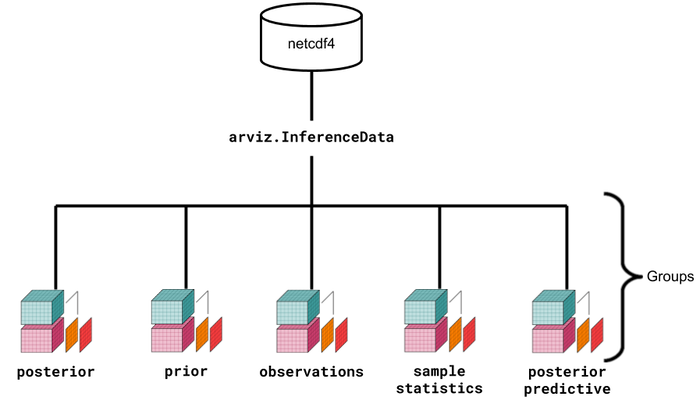
\includegraphics[width=0.6\linewidth]{InferenceDataStructure.png}
  \caption{Visual representation of the \texttt{InferenceData}
  structure.}\label{fig:data}
\end{figure}

\texttt{InferenceData} objects are central to ArviZ, most ArviZ functions
take \texttt{InferenceData} as input. Therefore, we provide functions
to convert between the outputs of several inference libraries and
\texttt{InferenceData}. Table~\ref{tab:from_xyz} shows the state of
converter functions in ArviZ beta release 0.6.1 (released in December 2019).
Natively supported libraries are PyStan, CmdStan and CmdStanPy
\cite{stan2018language, stan2018math, stan2018core, pystan2018}, % chktex 2
PyMC3~\cite{pymc32016}, Pyro and NumPyro~\cite{pyro2018},
emcee~\cite{emcee2013, emcee2019} and
TensorFlow Probability~\cite{tensorflow_probability2017}. In addition, there
is also a function to convert dictionaries of NumPy arrays to \texttt{InferenceData}.

\begin{table}[!ht]
  \caption{ArviZ converter functions summary}\label{tab:from_xyz}
  \begin{tabular}{ccccc}
    \toprule
    Inference library&Sampler stats&Posterior predictive&Observed data&Prior\\
    \midrule
    PyStan, CmdStan, CmdStanPy & \faCheck{} & \faCheck{} & \faCheck{} & \faCheck{} \\
    PyMC3 & \faCheck{} & \faCheck{} & \faCheck{} & \faCheck{} \\
    Pyro & \faCheck{}\footnote{For Pyro<1.0.0 there is only partial sampler
      stats support and no observed data available}
         & \faCheck{} & \faCheck\footnotemark[\value{footnote}] & \faCheck{} \\
    NumPyro & \faCheck{} & \faCheck{} & \faCheck{} & \faCheck{} \\
    emcee & Limited\footnote{emcee's blobs can be used to store sampler
    stats or even posterior predictive samples, however, blobs can store
  anything, so it is up to the user to customize them properly}
          & Limited\footnotemark[\value{footnote}]
          & \faCheck{} & \faTimes{} \\
    TensorFlow Probability & Limited\footnote{Only log likelihood data is
    retrieved} & \faCheck{} & \faCheck{} & \faTimes{} \\
  \bottomrule
\end{tabular}
\end{table}

Future design goals for \texttt{InferenceData} include two main goals:
support the storage of out-of-sample posterior predictive samples,
and storage of the arguments used
when calling the sampler as well as the kind of sampler. The latter goal
would allow reproducible sampling given the \texttt{InferenceData} object.

\section{Statistics and diagnostics}\label{sec:stats}
ArviZ includes many statistics and diagnostics for Bayesian
analysis such as the $\hat{R}$ statistic~\cite{gelman1992rhat, vehtari2019rank} or the
widely applicable information criterion~\cite{watanabe2010waic}.
We strive to provide sensible defaults for all algorithms and to
keep them up to date with the latest publications. Moreover, when installed,
Numba~\cite{lam2015numba} is optionally used to
speed up expensive calculations.

\subsection{Diagnostics}
Many convergence assessment functions are available in ArviZ.
\texttt{rhat}, \texttt{ess} and \texttt{mcse}
implement the $\hat{R}$ statistic, effective sample size and Monte Carlo
standard error respectively \cite{gelman1992rhat, gelman2013bayesian}. % chktex 2
The improvements in \citet{vehtari2019rank} have already been added to
ArviZ and have been made the default for all three functions. Moreover, all
three functions take
as input a method to choose between the available versions of the algorithms.
For example, the effective sample size can be calculated for the bulk, tail or for
quantiles and with or without rank normalization.
The \texttt{bfmi} function can be used to calculate Bayesian fraction
of missing information~\cite{betancourt2016diagnosing}, and the \texttt{geweke} function
implements z-scores for convergence diagnostics~\cite{geweke1991evaluating}.

A \texttt{summary} function is also provided for convenience to calculate
several diagnostics together with some statistics such as mean, standard deviation
or highest posterior density intervals.
Its output can be directly printed in a readable manner.

\subsection{Model comparison}
ArviZ also provides functions for model comparison using predictive
accuracy as metric. Given that ArviZ is intended to analysis of Bayesian
inference results and it aims to extend best practices, only fully
Bayesian algorithms have been implemented~\cite{gelman2014understanding}.
The \texttt{waic} function computes the
widely applicable information criterion~\cite{watanabe2010waic}, and the
\texttt{loo} function computes the leave one out cross validation using Pareto
smoothed importance sampling~\cite{vehtari2015pareto, vehtari2017practical}.

For iterative model building, the \texttt{compare} function can be used
to compute the WAIC or LOO value for several
models at the same time, effectively comparing them in a single line of code.

\subsection{Model checking}
One algorithm for model checking, the \texttt{loo\_pit} function, has also been implemented
recently: the leave
one out cross validation probability integral transform
(LOO-PIT)~\cite{gabry2019visualization}. This has been possible thanks to the
versatility of \texttt{InferenceData}, which contains all the quantities
needed for this calculation: observed data, posterior predictive samples and
log likelihood data. It should be noted that the LOO-PIT result is generally
analyzed visually in a qualitative way. This can also be done in ArviZ using
native plotting functions. Figure~\ref{fig:loo_pit} shows the difference
between the empirical cumulative density function (CDF) of the LOO-PIT values
and the CDF of a uniform distribution.

In addition, the results from \texttt{loo} and
\texttt{waic} functions can also be used for model checking to some extent.

\section{Data visualization}\label{sec:plots}
Many of the algorithms described in Section~\ref{sec:stats} have complementary
plots that extend them and ease their interpretability. Some
examples are \texttt{plot\_compare}, \texttt{plot\_loo\_pit} or
\texttt{plot\_ess} which complement the algorithms of the same name, but
also \texttt{plot\_khat} to complement \texttt{loo}, or
\texttt{plot\_elpd} to complement either \texttt{waic} or
\texttt{loo}.

ArviZ provides plotting functions suited to many different tasks:
visualization of probabiliy distributions, model checking, convergence
diagnostics, or model comparison. The
documentation contains an
\href{https://arviz-devs.github.io/arviz/examples/index.html}{example
gallery}\footnote{\url{https://arviz-devs.github.io/arviz/examples/index.html}}
showcasing all plots currently available in ArviZ. Figure~\ref{fig:examples}
shows some of the recently added plots.

Additionally, the plots may use either Matplotlib~\cite{Hunter2007matplotlib},
which is versatile and well
tested, especially for preparing static plots, or Bokeh~\cite{bokeh}, which allows for
interactivity and web-based graphics.

\begin{figure}[!htb]
\centering
  \begin{subfigure}{.47\textwidth}
  \centering
    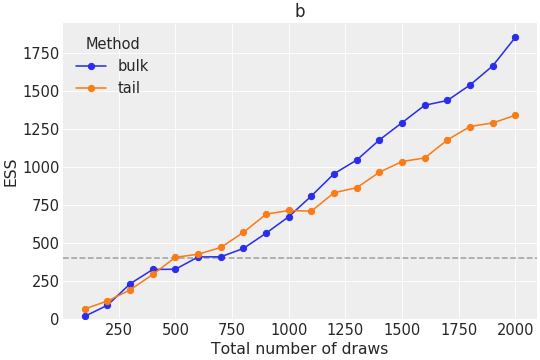
\includegraphics[width=\linewidth]{plot_ess.png}
    \caption{Evolution of the effective sample size as the sample size
    increases. A non-linear evolution of the effective sample size
    indicates convergence problems~\cite{vehtari2019rank}.}
  \end{subfigure}
  \begin{subfigure}{.47\textwidth}
  \centering
    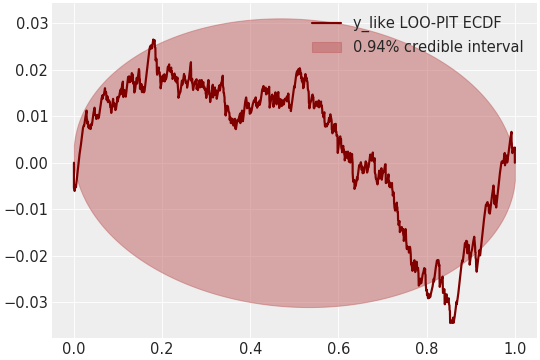
\includegraphics[width=\linewidth]{plot_loo_pit.png}
    \caption{Difference between LOO-PIT empirical CDF and a uniform
      distribution. Differing
      from a uniform distribution indicates model
      mispecification~\cite{gabry2019visualization}.}\label{fig:loo_pit}
  \end{subfigure}\\
  \begin{subfigure}{0.98\textwidth}
  \centering
    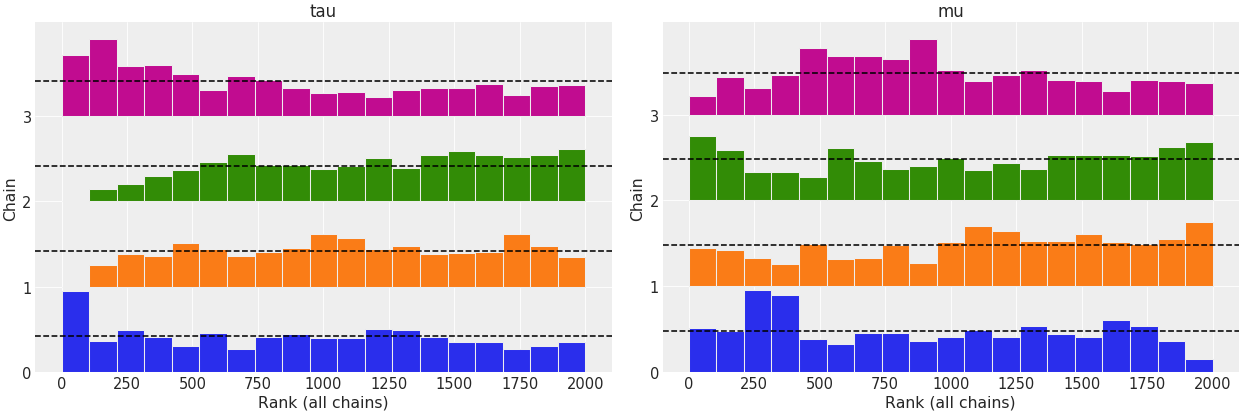
\includegraphics[width=\linewidth]{plot_rank.png}
    \caption{Rank plots are an alternative to the commonly used trace
      plots~\cite{vehtari2019rank}.}\label{fig:n2}
  \end{subfigure}
  \caption{Examples of plotting functions added to ArviZ during
  2019.}\label{fig:examples}
\end{figure}

\section*{Funding}
Work by Osvaldo Martin was supported by CONICET-Argentina and ANPCyT-Argentina
(PICT-0218). Two students were funded by the Google Summer of Code project to
work on ArviZ between May and August 2019. In addition, a NumFOCUS small
development grant was awarded to ArviZ.

\begin{acks}
  We would like to acknowledge all the communities involved in ArviZ
  development ---especially Adrian Seyboldt, Junpeng Lao,
  Thomas Wiecki, and Robert Goldman from the PyMC community, Allen Riddell and
  Aki Vehtari from the Stan community, and Du Phan from the Pyro community.
  We also would like to thank everyone who contributed to ArviZ by sending pull
  requests or posting issues ---especially Aniruddha Banerjea for his work
  during Google Summer of Code---, and the contributors of the libraries used to
  build ArviZ ---particularly xarray, Matplotlib, Bokeh, pandas, and NumPy. We
  also thank NumFOCUS for supporting ArviZ as an affiliated project.
\end{acks}

\bibliographystyle{acm-reference-format}
\bibliography{probprog-2020-proposal}

% \appendix
% \section{Appendices}

\end{document}
